\chapter{Управление по прогнозируемой модели в model-based обучении с подкреплением}\label{chap4}

%%%%%%%%%%%%%%%%%%%%%%%%%%%%%%%%%%%%%%%%%%%%%%%%%%%%%%%%%%%%%%%%%%%%%%%%%%%%%%%%
\section{Марковский процесс принятия решений для в рамках управления с прогнозирующими моделями}\label{1sec:optimal-control}
%%%%%%%%%%%%%%%%%%%%%%%%%%%%%%%%%%%%%%%%%%%%%%%%%%%%%%%%%%%%%%%%%%%%%%%%%%%%%%%%


В рамках управления по прогнозируемой модели в задачах оптимального управления с ограничениями марковский процесс принятия решений несколько трансформируется. Кроме перечисленных в главе 2 характеристик (состояние среды, множество возможных действий, модель среды, функции наград) к нему добавляется функция стоимости $c: S \to \{0, 1\}$. Она является индикатором, где 0 значит, что ограничения выполнены, а 1 -- нарушены. 

В рамках данного подхода мы считаем, что модель среды (функции (\ref{eq:psi}) и (\ref{eq:phi})) и функция стоимости неизвестны и должны быть найдены на основе собранных данных. Пусть $J_r (\pi)$ обозначает ожидаемую доходность при политике $\pi$ относительно функции вознаграждения $r$, а $J_c (\pi)$ -- доходность при политике $\pi$ относительно функции стоимости $c$:

\begin{equation}
	J_r(\pi) = E_{\pi}[\sum\lim_{t=0}^{T-1} r(s_{t+1})],
	\label{eq:jr}
\end{equation}
\begin{equation}
    J_c(\pi) = E_{\pi}[\sum\lim_{t=0}^{T-1} c(s_{t+1})],
    \label{eq:jc}
\end{equation}
где $T$ -- это горизонт планирования. 

Как было сказано выше, основная цель -- максимизировать ожидаемую доходность (\ref{eq:doh}). При наложенных ограничениях задача состоит в том, чтобы максимизировать ожидаемую доходность  относительно вознаграждения и ограничить ожидаемую доходность относительно функции стоимости. В общем виде это может быть записано следующим образом:

\begin{equation}
	\begin{split}
		\pi^* = \arg \max_{\pi} J_r(\pi), \\
		J_c(\pi^*) \leq d,
	\label{eq:task3}
	\end{split}
\end{equation}
где $d$ -- заданный лимит на количество нарушений ограничений, а функции $J_r(\pi)$ и $J_c(\pi)$ заданы по формулам (\ref{eq:jr}) и (\ref{eq:jc}) соответственно. 


%%%%%%%%%%%%%%%%%%%%%%%%%%%%%%%%%%%%%%%%%%%%%%%%%%%%%%%%%%%%%%%%%%%%%%%%%%%%%%%%
\section{Управление с прогнозирующими моделями (MPC)}\label{1sec:optimal-control}
%%%%%%%%%%%%%%%%%%%%%%%%%%%%%%%%%%%%%%%%%%%%%%%%%%%%%%%%%%%%%%%%%%%%%%%%%%%%%%%%


Напомним, что как следует из главы 1 в основе MPC лежат два основных принципа:
\begin{enumerate}
	\item Использовать динамическую модель для предсказания состояния системы и улучшения предсказания для принятия оптимального решения -- \textit{управления} в текущий момент времени.
	
	\item Использовать предыдущие состояния системы для инициализации состояния динамической модели.
\end{enumerate}

Также напомним, что MPC применяется для решения задач стабилизации и в этом случае выбираются специальные критерии качества, которые на оптимальном значении представляет собой функцию Лапунова для стабилизируемой системы. Прогнозируемая задача оптимального управления в данном случае -- задача на минимум.

В терминах исследуемой задачи цель MPC — максимизировать суммарную награду (\ref{eq:doh}), выбирая последовательность действий $U=(a_0, \dots, a_T)$, где $T$ -- это горизонт планирования. За один шаг к системе применяется оптимальное управление (действие) и  получаются новые наблюдения, после чего заново пересчитываются следующие оптимальные действия. Таким образом находясь в состоянии $s_t$ в момент времени $t$ целью MPC является найти:

\begin{equation}
	\begin{split}
	U = \arg \max_{a_0, a_1, \dots, a_T} [ \mathbb{E}  \sum \limits_{t=0}^{T} \gamma^t r(s_{t+1})] , \\
	c(s_{t+1}) = 0, \\
	\forall t \in {0, 1, \dots, T-1}. 
	\label{eq:U}
	\end{split}
\end{equation}


Визуально представить себе работу управления по прогнозирующей модели можно так, как показано на рисунке ~\ref{fig:mpc-ex}. \newpage

\begin{figure}[h]
	\centering
	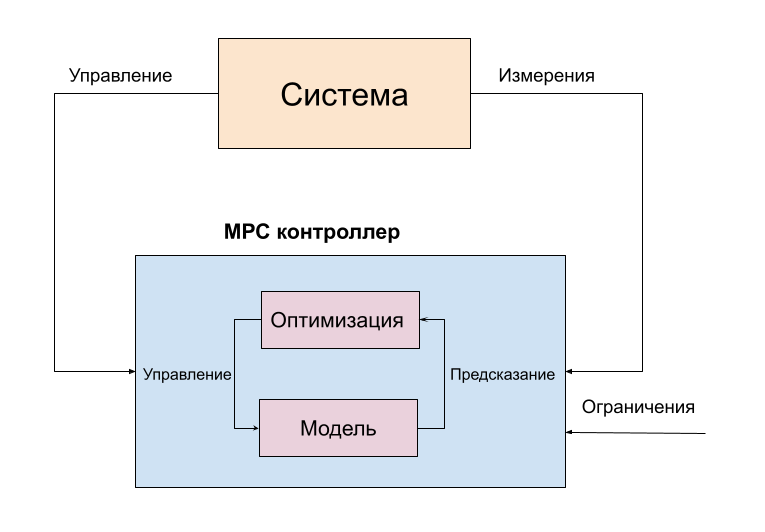
\includegraphics[scale=0.7]{mpc_ex.png}
	\caption{МРС}\label{fig:mpc-ex}
\end{figure}




%%%%%%%%%%%%%%%%%%%%%%%%%%%%%%%%%%%%%%%%%%%%%%%%%%%%%%%%%%%%%%%%%%%%%%%%%%%%%%%%
\section{Model-based обучение с подкреплением}\label{1sec:optimal-control}
%%%%%%%%%%%%%%%%%%%%%%%%%%%%%%%%%%%%%%%%%%%%%%%%%%%%%%%%%%%%%%%%%%%%%%%%%%%%%%%%

В данный момент существует два основных подхода в обучении с подкреплением: model-based и model-free. Основное их отличием является взаимодействие ос средой и представление о ней. Model-free алгоритмы обучаются на собственном опыте при запуске в реальной среде для обучения (компьютерные игры, реальный мир). Подход model-based же контактирует с реальной средой намного меньше и на этапе обучения старается заменить ее собственным аналогом среды. Таким образом одной из основных задач model-based алгоритмов является построение качественной модели среды (\ref{eq:model}).

Как было сказано в предыдущем разделе, в рамках исследуемой задачи один из способов решения будет основан на отсутствии знаний о среде. Таким образом мы должны получить представление о ней. А именно аппроксимировать функции (\ref{eq:psi}) и (\ref{eq:phi}) и получить модель (\ref{eq:model}). Это происходит на основе генерации выборок из реальной среды. В качестве аппроксимации  модели среды (\ref{eq:model}) часто используется нейронная сеть.

Полный цикл обучения модели и работы управления с прогнозирующими моделями представлен на рисунке ~\ref{fig:mpc-m}. \newpage
 
 
 \begin{figure}[h]
 	\centering
 	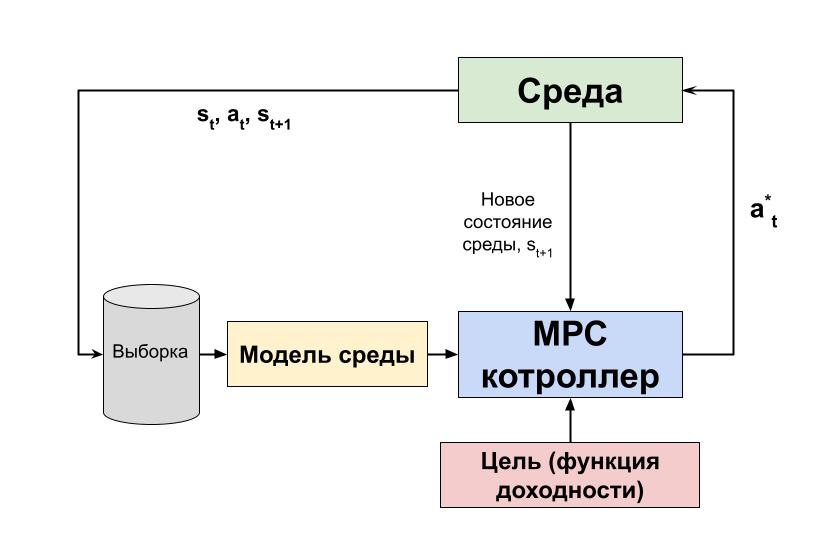
\includegraphics[scale=0.6]{mpc_model.png}
 	\caption {Модель обучения MPC}
 	\label{fig:mpc-m}
 \end{figure}





%%%%%%%%%%%%%%%%%%%%%%%%%%%%%%%%%%%%%%%%%%%%%%%%%%%%%%%%%%%%%%%%%%%%%%%%%%%%%%%%
\section{Метод кросс-энтропии для задач оптимизации}\label{1sec:optimal-control}
%%%%%%%%%%%%%%%%%%%%%%%%%%%%%%%%%%%%%%%%%%%%%%%%%%%%%%%%%%%%%%%%%%%%%%%%%%%%%%%%

Метод кросс-энтропии (CEM) это метод стохастической оптимизации, основанный на генерации выборок (сэмплировании траекторий, СТ) \cite{cem2}. С недавнего времени он часто используется в задачах обучения с подкреплением. В рамках данного метода предполагается, что $T$-размерное решение $U \in R^T$ (\ref{eq:U}) получено из $T$-размерного факторизированного многомерное распределение Гаусса с параметром $\theta$.

Тогда мы имеем выборку $U \sim N(\theta)$, где $\theta = (\mu, \Sigma)$, $\mu$ --  $T$-вектор, а $\Sigma$ -- диагональная $T x T$ матрица ковариаций.

Основная идея метода заключается в том, чтобы генерировать решения итеративно из распределения, которое близко к распределению, из которого получены предыдущие сгенерированные результаты с высокой наградой. Алгоритм останавливается, если достигнуто максимальное количество итераций или $|\Sigma| > \epsilon$, где $\epsilon$ -- заданный фиксированный порог на матрицу ковариаций. 

Одним из способов решения исследуемой задачи оптимизации (\ref{eq:task3}) является робастный метод кросс-энтропии (RCE), основанный на методе кросс-энтропии. Он базируется на  методе сэмплирования траекторий (СТ)  \cite{cem1} для оценки вознаграждения и стоимости нарушения ограничений. Определим решение (\ref{eq:U}) как последовательность действий размера 
горизонта планирования $T$ :
 $$U = (a_0, a_1, ..., a_{T −1}).$$  
 
При начальном состоянии $s_0$ , модели среды $m_{\theta}(s_t, a_t)$ (\ref{eq:model}), функции стоимости  $c(s) \in {0, 1}$, мы можем оценить накопленное вознаграждение следующим образом:
\begin{equation}
	r(X, s_0) = \sum\limits_{t=0}^T \gamma^t r(s_{t+1}),
	\label{eq:r}
\end{equation}

\begin{equation}
	c(X, s_0) = \sum\limits_{t=0}^T \beta^t c(s_{t+1}),
	\label{eq:c}
\end{equation}
 где $s_{t+1} = m_{\theta}(s_t, a_t), \forall  t \in \{0, \dots, T-1\}$ (\ref{eq:model}), $\gamma$ и $\beta$ -- дисконтирующие множители. Данные формулы являются аппроксимацией формул (\ref{eq:jr}) и (\ref{eq:jc}) для решения задачи (\ref{eq:task3}) в рамках управления по прогнозируемой модели.

Награда $r(s)$ может быть либо предопределенной, заранее функцией, либо изучена параллельно с моделью.  

Интуитивное представление о работе данного метода на примере задачи о роботе показано на рисунке ~\ref{fig:cross-ent}. Точки на синей линии и точки на оранжевой линии представляют собой две реальные траектории, эллипсы
представляют собой неопределенность прогноза модели среды на основе наблюдений и последовательности действий. На рисунке видно, что награда за траекторию B должна быть выше, чем за траекторию A, потому что выбор B приведет к в достижению цели быстрее. Однако траектория A предпочтительнее, потому что робот, следующий по траектории B, может пройти
через пламя и нарушить ограничения безопасности.


\begin{figure}[h]
	\centering
	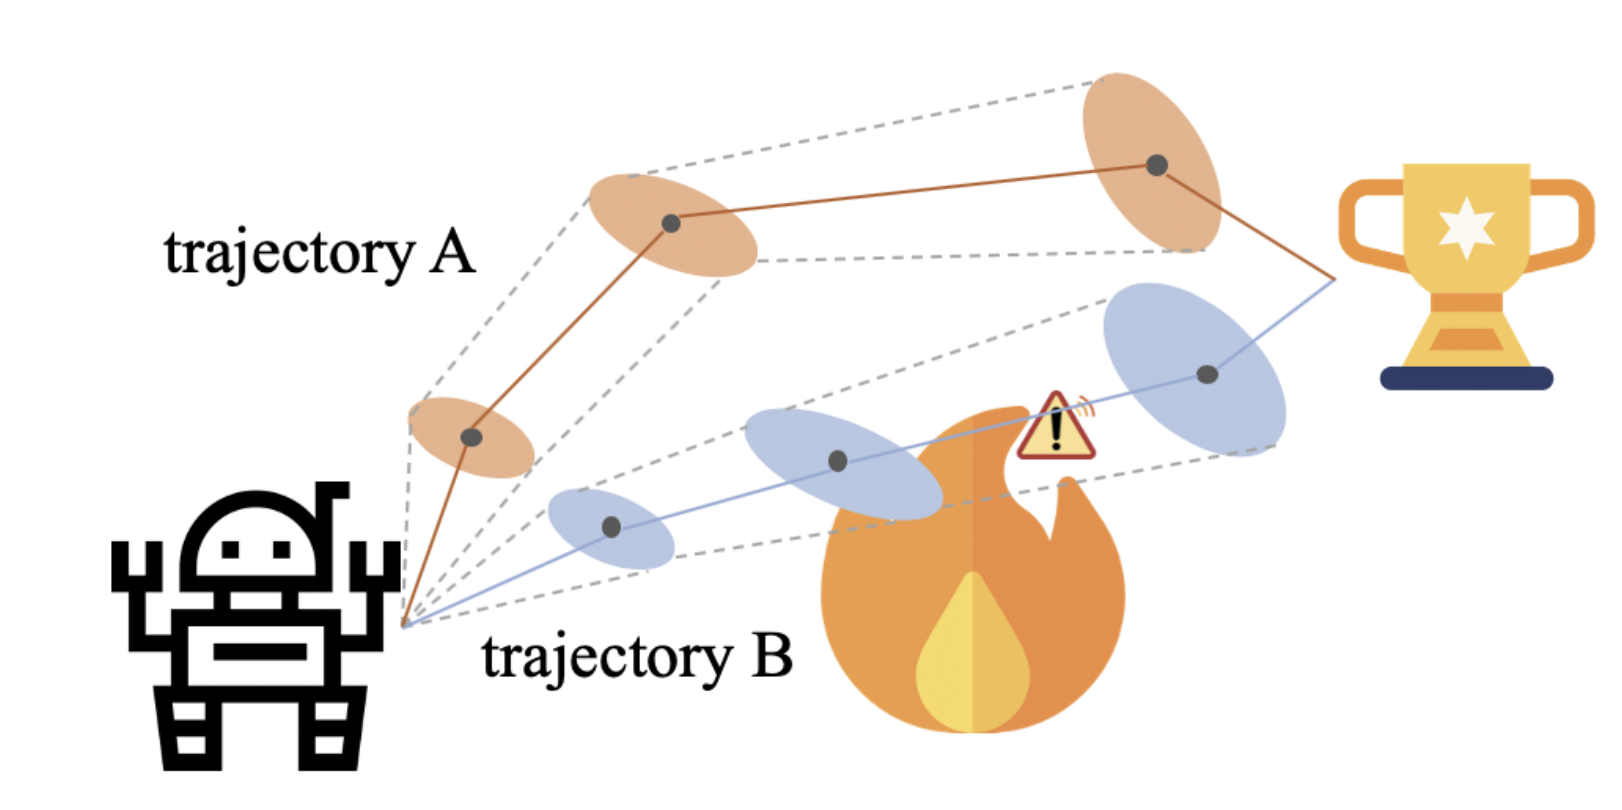
\includegraphics[scale=0.6]{cem_alg.png}	
	\caption {Метод кросс-энтропии}
	\label{fig:cross-ent}
\end{figure}


Без сэмплирования траекторий, траектория B потенциально может быть предсказана как безопасный маршрут из-за ошибки прогноза модели.  С СТ,
оценка неопределенности нашей модели имеет небольшой
шанс охватить небезопасную зону, поэтому траектория B будет
классифицироваться как небезопасная. Поскольку СТ оценивает стоимость
траектории при наихудшем сценарии среди всех отобранных маршрутов, он более надежен, когда прогноз модели среды не очень точный.


Обозначим функцию плотности распределения как $p(U, \theta)$. 
Тогда алгоритм состоит из следующих шагов: 
\begin{enumerate}
	\item Выбираем набор решений.
	\item Считаем для него функции $r, c$ по формулам (\ref{eq:r}) и (\ref{eq:c})
	\item Проверяем достижимы ли данные решения. 
	\item Пересчитываем параметры распределения на основе лучших $k$ решений.
\end{enumerate}

Псевдокод описанного выше алгоритма выглядит следующим образом: 
\begin{algorithm}
	\caption{Метод робастной кросс-энтропии}\label{cem}
	\begin{algorithmic}[1]
		\State{Начальная инициализация параметра распределения $\theta$, размерность выборки $T$, количества отбираемых элементов из выборки $k$, начального состояния $s_0$.}
		\State{Генерация выборки $U$  с высокой наградой}
		
		\While{Критерий остановки  не выполнен}
		\State{Сгенерировать $N$ примеров из исходного распределения $U_1, U_2, \dots, U_N  \sim N(\theta)$.}
		\State{Для каждого элемента выборки $U_i$ вычислить $r(U_i, s_0)$ и $c(U_i, s_0)$.}
		\State{Выбрать подходящее подмножество элементов $\Omega \in \{U_i \}_{i=1}^N$ не нарушающих ограничения на основе функции стоимости.}
		\If{$\Omega = \emptyset$ -- пустое множество} 
		\State{Отсортировать $\{U_i\}_{i=1}^N$ в порядке убывания по функции стоимости; задать множество $\Delta_k$ -- из топ $k$ элементов после сортировки}
		\Else{}
		\State{Отсортировать множество $\Omega$ в порядке убывания по награде. Задать множество $\Delta_k$ из первых $k$ элементов, если $|\Omega| > k$, или $\Delta_k = \Omega$}.
		\EndIf
		\State{Обновить $\theta$ с помощью метода максимального правдоподобия: $\theta = arg \max_{\theta} \prod_{U \in \Delta_k} p(U, \theta)$.}
		\EndWhile
		\State{Вернуть $U^*$ с самой высокой наградой из $\Delta_k$.}
	\end{algorithmic}
\end{algorithm}
\bigskip

Для исследуемой задачи мы будем использовать модернизированный робастный метод кросс-энтропии. А именно кроме поиска набора управления $U$  с помощью алгоритма 1, описанного выше, мы параллельно будем обучать модель среды (\ref{eq:model}) и функцию стоимости $c(s_{t+1})$. Псевдокод для нашего алгоритма можно увидеть ниже:\newpage

\begin{algorithm}
	\caption{Метод робастной кросс-энтропии}\label{cem}
	\begin{algorithmic}[1]
		\State{Начальная генерация выборки $D=\{s_1, a_1, \dots, s_N, a_N\}$, инициализация параметра $p(U, \theta)$.}
		
		\While{Количество итераций меньше максимального}
		\State{Тренировать модель среды $m(s_t, a_t)$ и функцию стоимости $c$ на основе выборки $D$.}
		\For{t=0 до конца длины эпизода }
		\State{Получить состояние среды $s_t$}
		\State{Оптимизировать действие согласно алгоритму 1: \\ $\{a_{i^*}\}_{i=t}^{t+T} = RCE(p, s_t)$}
		\State{Выбрать действие и подать его в систему }
		\State{Получить из среды следующее состояние $s_{t+1}$ и функцию стоимости $c(s_{t+1})$}
		\State{Обновить выборку $D=D \bigcup \{ s_t, a_t, s_{t+1}, c(s_{t+1})\}$.}
		
		\EndFor
		\EndWhile
		\State{Вернуть $X^*$ с самой высокой наградой из $\Delta_k$.}
	\end{algorithmic}
\end{algorithm}

%%%%%%%%%%%%%%%%%%%%%%%%%%%%%%%%%%%%%%%%%%%%%%%%%%%%%%%%%%%%%%%%%%%%%%%%%%%%%%%%
\section{Выводы}\label{1sec:optimal-control}
%%%%%%%%%%%%%%%%%%%%%%%%%%%%%%%%%%%%%%%%%%%%%%%%%%%%%%%%%%%%%%%%%%%%%%%%%%%%%%%%


В данной главе представлена теория model-based подхода для решения задач оптимального управления. Описана общая теория управления по прогнозируемой модели. Приведен алгоритм кросс-энтропии для построения горизонта управления и его усовершенствование -- метод робастной кросс-энтропии.


%В обучении с подкреплением же это означает наличие представления о среде $M$ для MDP $(S, A, P, \gamma,  R)$. А именно наличие версии модели окружающей среды в момент времени $i$ для Марковского процесса принятия решений.  

%Таким образом при известном пространстве состояний $S$ и вероятности переходов $A$, модель $M_i$ будет выглядеть как $M_i(S, A, P_i,\gamma,  R_i)$. И это значит, что, согласно модели вероятность перехода из состояния $S$ в $S ‘$ после выполнения действия $A$ равна $P_i (S' | S, A)$, аналогично вознагражение, полученное в результате действия $A$  в состоянии $S$  равно $R_i (r '| S,  A)$.


